\begin{appendices}
\chapter{Chroma Subsampling Artefakte}
\label{appendix:subsampling_artefacts}
\begin{figure}[h!]
    \centering
    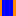
\includegraphics[scale=10]{images/2-1_chroma_artefacts_original.png}
    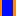
\includegraphics[scale=10]{images/2-1_chroma_artefacts_sampled.png}
    \caption{Artefakte durch Chroma Subsampling}
    \textit{Links: Original, Rechts: Subsampled. Die rechte Kante des blauen Farbblocks liegt in gesubsampleten 2x2 Blöcken, wodurch Artefakte entstehen. Die linke Kante liegt zwischen zwei 2x2 Blöcken, weshalb es zu keiner falschen Darstellung kommt.}
    \label{fig:chroma_artefacts}
\end{figure}

\chapter{Quantisierung}
\label{appendix:qauntisierung}

\begin{figure}[h!]
    \centering
    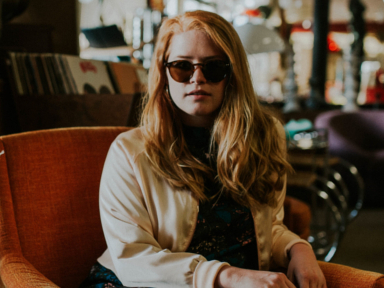
\includegraphics[scale=0.5]{images/2-3_brook_orig.png}
    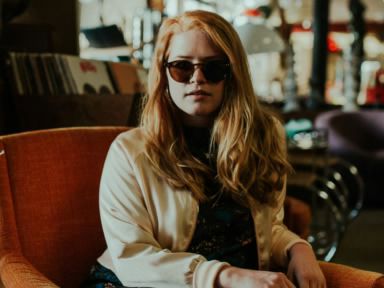
\includegraphics[scale=0.5]{images/2-3_brook_1.png}
    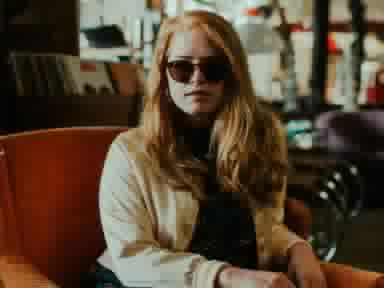
\includegraphics[scale=0.5]{images/2-3_brook_16.png}
    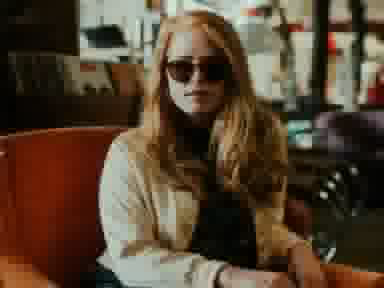
\includegraphics[scale=0.5]{images/2-3_brook_31.png}
    \caption{Ergebnis der Quantisierung mit verschiedenen Quantisierungsfaktoren}
    \textit{Oben links: Original, Oben rechts: Quantisiert mit Faktor 1, Unten links: Quantisiert mit Faktor 16, Unten rechts: Quantisiert mit Faktor 31.\\
    Mit zunehmendem Quantisierungsfaktor ist ein ansteigender Verlust der Bildqualität zu beobachten, wobei grobe Strukturen weitestgehend erhalten bleiben. Original nach \cite{brooke_cagle__2016}}
    \label{fig:chroma_artefacts}
\end{figure}
\end{appendices}
